%!TEX root=ast2016.tex

\begin{figure*}[t]
  \centering

  \begin{tabular}{c c}

    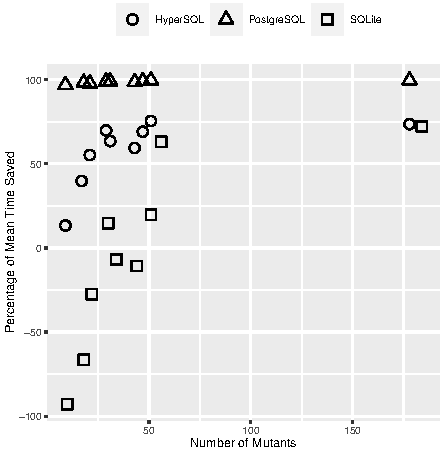
\includegraphics[scale=1.0]{graphics/graphic_scatterplot_nummutants_percentage.pdf} &
    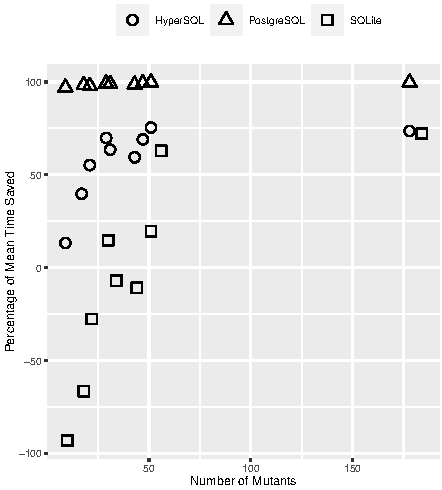
\includegraphics[scale=1.0]{graphics/graphic_scatterplot_numtests_percentage.pdf}

  \end{tabular}

  \caption{Scatter plot of the percentage of mean time saved for the number of mutants (left) and tests (right).}
  \label{fig:graphic_scatterplot_mutantstests_percentagetimesaved}

  {\small \justifying{ \noindent In these scatter plots, a given point corresponds to the percentage of mean time saved
      for a given number of mutants (left plot) or tests (right plot), across all three of the DBMSs.  The percentage of
      mean time saved is determined by first calculating the mean execution time from the thirty trials of both the
      standard and the virtual techniques. If $T_s$ denotes the mean time taken by the standard method and $T_v$ is the
      mean time needed for the virtual one, then the percentage of mean time saved shown on the vertical axis is given by
  $({T_s - T_v})/{T_s}$. } \par}

\end{figure*}
